\chapter{Los registros existentes}\label{sec:chapterVI}
\addcontentsline{toc}{chapter}{Los registros existentes}

A continuación se realizará un análisis del dataset del que disponemos con el fin de asegurar su fiabilidad y homogeneidad. Es decir, se comprobará la normalidad del mismo año tras año.

En el laboratorio remoto se ha registrado la actividad de $7$ años consecutivos (desde el curso académico $1516$ al $2122$). Un ejemplo de las interacciones almacenadas puede verse en el Cuadro \ref{tab:example}.

\begin{table}[H]
\centering
\caption{Muestra de los datos que se recopilan en el servidor.}
\label{tab:example}
\begin{tabular}{cccccc}
\hline
\textbf{Year} & \textbf{Group} & \textbf{SessionID} & \textbf{Date}       & \textbf{Problem} & \textbf{Step} \\ \hline
1819          & Keid           & 493252533735       & 28/10/2018 20:23:35 & P1               & 1             \\ 
1819          & Keid           & 493252533735       & 28/10/2018 20:23:40 & P1               & 3             \\ 
1819          & Keid           & 389034076811       & 7/11/2018 19:01:49  & P2               & 1             \\
1819          & Cerastes       & 487544594557       & 27/10/2018 13:05:11 & P1               & 1             \\
1819          & Cerastes       & 487544594557       & 27/10/2018 13:10:57 & P1               & 3             \\
1819          & Jabbah         & 550676318711       & 20/12/2018 22:22:42 & P8               & 1             \\
1819          & Cerastes       & 336303012053       & 17/12/2018 13:28:50 & P9               & 1             \\ 
1819          & Keid           & 563159878397       & 25/10/2018 12:41:43 & P8               & 1             \\ \hline
\end{tabular}
\end{table}

\section{Número de grupos cada año}

El número de grupos puede variar en cada curso en función del número de alumnos matriculados en la asignatura ese año. Así pues, se muestran a continuación en los Cuadros \ref{tab:groups1} y \ref{tab:groups2} los grupos por curso académico. El número de grupos por año puede consultarse también en la Figura \ref{fig:groupsperyear}.

\begin{figure}[H]
    \centering
    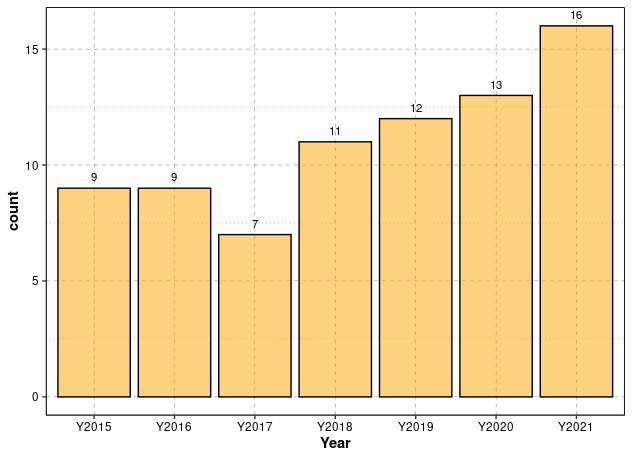
\includegraphics[width=0.6\textwidth]{análisis/numregistersyear.png}
    \caption{Número de grupos por curso académico estudiado.}
    \label{fig:groupsperyear}
\end{figure}

\section{El periodo de tiempo analizado cada año}

En el Cuadro \ref{tab:days} se muestra el número de días que dura la práctica cada año. Se puede apreciar que la duración de la práctica que estamos considerando puede variar en función del curso académico.

\begin{table}[H]
\centering
\caption{Número de días que dura la práctica cada año.}
\label{tab:days}
\begin{tabular}{cc}
\hline
\textbf{Year}  & \textbf{Length (days)}  \\ \hline
Y2015 & 32 \\
Y2016 & 23 \\
Y2017 & 29 \\
Y2018 & 17 \\
Y2019 & 27 \\
Y2020 & 16 \\
Y2021 & 38 \\ \hline
Mean & 26 \\
SD & 7.958224 \\ \hline
\end{tabular}
\end{table}

\section{El conjunto de problemas analizados cada año}

Todos los años hay $9$ problemas de dificultad similar que deben ser resueltos por todos los grupos.

Para aproximarnos al concepto subjetivo de ``dificultad del problema'' vamos a analizar el número de sesiones fallidas que necesita cada alumno para resolverlos por primera vez con respecto al número total de sesiones de ese problema (tasa de fallo) y la duración de este periodo en horas para determinar si realmente hay diferencias en la dificultad de los problemas planteados.

\subsection{Dificultad del problema: la tasa de fallo}

La apertura de un problema se corresponde con una sesión de trabajo, la cual puede terminar fracasando (fail) si no se consigue resolver el problema, o teniendo éxito (solved) en caso de que se haya resuelto el problema. Así pues, se definirá la tasa de fallo como el cociente entre el número total de sesiones fallidas y el número total de sesiones de un mismo problema. El boxplot de las tasas de fallo por problema puede verse en la Figura \ref{fig:boxplotfailratio}. En él, podemos observar que, aunque al principio cuesta empezar (la tasa de fallo del segundo problema es en media mayor que la del primero), los problemas $3$, $4$ y $5$ se resuelven con mayor facilidad y podrían considerarse equivalentes en cuanto a dificultad. Nótese, además, que la práctica está aprobada si se resuelven los cinco primeros problemas de la misma. Por otro lado, los cuatro últimos problemas presentan una dificultad creciente y superior a la de los cinco primeros problemas y determinarán la nota de la práctica. Esta tendencia primero decreciente y luego creciente se ha creado de manera intencionada por parte del profesorado para motivar al alumnado al principio de la práctica y empujarles a resolver los últimos problemas al final de la misma.

\begin{figure}[H]
    \centering
    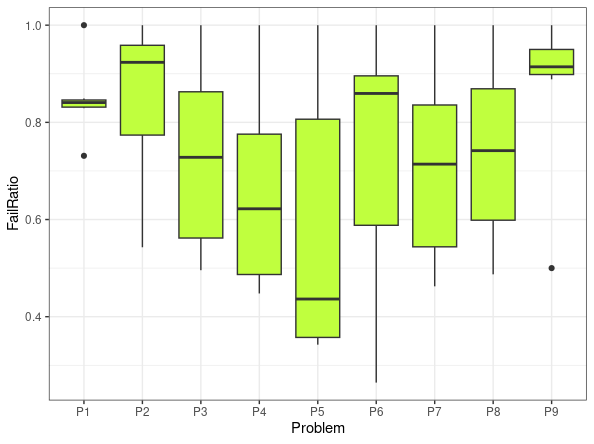
\includegraphics[width=0.8\textwidth]{análisis/boxplotfailratioproblem.png}
    \caption{Boxplot de la tasa de fallo (\emph{fail ratio}) por problema.}
    \label{fig:boxplotfailratio}
\end{figure}

Tras realizar el test ANOVA de un factor (resultados en el Cuadro \ref{tab:ANOVAfailratio}), cuya hipótesis nula establece que la tasa de fallo media de los nueve problemas considerados es la misma, se detecta que las diferencias entre las distribuciones de probabilidad de la tasa de fallo  podrían ser estadísticamente significativas en los distintos problemas ($p = 7.72e-12 < 0.05$)\footnote{Nótese que hemos establecido un nivel de significancia de $\alpha = 0.05$.}. Si aplicamos el test de Kruskal-Wallis, obtenemos $p-value = 3.756e-12 < 0.05$, lo que confirma los resultados obtenidos por el test de ANOVA.

% latex table generated in R 4.3.1 by xtable 1.8-4 package
% Wed Aug  2 16:49:26 2023
\begin{table}[H]
\centering
\caption{Resultados del test ANOVA de un solo factor (tasa de fallo).}
\label{tab:ANOVAfailratio}
\begin{tabular}{lrrrrr}
  \hline
 & Df & Sum Sq & Mean Sq & F value & Pr($>$F) \\ 
  \hline
fr & 8 & 4.00 & 0.50 & 9.12 & 7.72e-12 \\ 
  Residuals        & 570 & 31.23 & 0.05 &  &  \\ 
   \hline
\end{tabular}
\end{table}

Además, se ha realizado un test de Tukey por pares de problemas (Cuadro \ref{tab:Tukeyfailratio}). En él se observa que no todos los pares pueden considerarse estadísticamente iguales aunque haya algunos que quizá puedan serlo, como el par $P1-P2$ ($\text{p adj} = 1.00$). La Figura \ref{fig:confidenceratiofail} muestra los intervalos de confianza de todas las diferencias entre las distintas parejas de años.

\begin{table}[H]
\centering
\caption{Test HSD de Tukey (Honestly-significance-difference) de la tasa de fallo por problemas.}
\label{tab:Tukeyfailratio}
\begin{tabular}{rrrrr}
  \hline
 & diff & lwr & upr & p adj \\ 
  \hline
p2-p1 & -0.00 & -0.13 & 0.12 & 1.00 \\ 
  p3-p1 & -0.11 & -0.24 & 0.01 & 0.11 \\ 
  p4-p1 & -0.17 & -0.29 & -0.04 & 0.00 \\ 
  p5-p1 & -0.22 & -0.35 & -0.10 & 0.00 \\ 
  p6-p1 & -0.08 & -0.21 & 0.04 & 0.47 \\ 
  p7-p1 & -0.09 & -0.21 & 0.03 & 0.36 \\ 
  p8-p1 & -0.06 & -0.18 & 0.06 & 0.81 \\ 
  p9-p1 & 0.08 & -0.05 & 0.21 & 0.61 \\ 
  p3-p2 & -0.11 & -0.24 & 0.02 & 0.17 \\ 
  p4-p2 & -0.16 & -0.29 & -0.03 & 0.00 \\ 
  p5-p2 & -0.22 & -0.35 & -0.09 & 0.00 \\ 
  p6-p2 & -0.08 & -0.21 & 0.05 & 0.59 \\ 
  p7-p2 & -0.08 & -0.21 & 0.04 & 0.48 \\ 
  p8-p2 & -0.06 & -0.18 & 0.07 & 0.89 \\ 
  p9-p2 & 0.08 & -0.05 & 0.22 & 0.57 \\ 
  p4-p3 & -0.05 & -0.19 & 0.08 & 0.95 \\ 
  p5-p3 & -0.11 & -0.24 & 0.02 & 0.20 \\ 
  p6-p3 & 0.03 & -0.10 & 0.16 & 1.00 \\ 
  p7-p3 & 0.03 & -0.10 & 0.15 & 1.00 \\ 
  p8-p3 & 0.05 & -0.08 & 0.18 & 0.94 \\ 
  p9-p3 & 0.19 & 0.06 & 0.33 & 0.00 \\ 
  p5-p4 & -0.06 & -0.19 & 0.08 & 0.93 \\ 
  p6-p4 & 0.08 & -0.05 & 0.22 & 0.57 \\ 
  p7-p4 & 0.08 & -0.05 & 0.21 & 0.64 \\ 
  p8-p4 & 0.10 & -0.03 & 0.24 & 0.24 \\ 
  p9-p4 & 0.25 & 0.11 & 0.38 & 0.00 \\ 
  p6-p5 & 0.14 & 0.01 & 0.27 & 0.03 \\ 
  p7-p5 & 0.13 & 0.01 & 0.26 & 0.03 \\ 
  p8-p5 & 0.16 & 0.03 & 0.29 & 0.00 \\ 
  p9-p5 & 0.30 & 0.17 & 0.44 & 0.00 \\ 
  p7-p6 & -0.01 & -0.13 & 0.12 & 1.00 \\ 
  p8-p6 & 0.02 & -0.11 & 0.15 & 1.00 \\ 
  p9-p6 & 0.16 & 0.03 & 0.30 & 0.01 \\ 
  p8-p7 & 0.03 & -0.10 & 0.15 & 1.00 \\ 
  p9-p7 & 0.17 & 0.03 & 0.30 & 0.00 \\ 
  p9-p8 & 0.14 & 0.01 & 0.27 & 0.03 \\ 
   \hline
\end{tabular}
\end{table}

\begin{figure}[H]
    \centering
    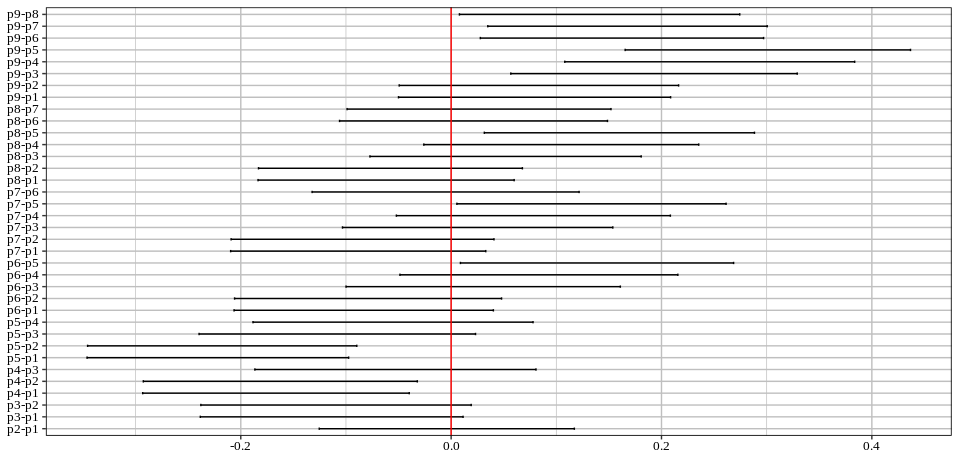
\includegraphics[width=0.80\textwidth]{análisis/confidencefailratio.png}
    \caption{Intervalos de confianza de la tasas de fallo de los problemas.}
    \label{fig:confidenceratiofail}
\end{figure}

Estos datos hay que interpretarlos de manera incremental, pues para resolver un problema $P_i$ se requieren las habilidades de los problemas $P_j$, $0\leq j < i$ más habilidades nuevas propias del problema $P_i$. Así pues, periódicamente se incrementa notablemente el nivel de dificultad. % P1 es el que más cuesta porque siempre cuesta trabajo empezar, P2-4 son muy parecidos y P5 es un poco más difícil, P6-P8 suben un escalón de dificultad y P9 también.

\subsection{Dificultad del problema: tiempo necesario en resolverlo}

Es el número de horas que transcurren desde que el problema se abre por primera vez hasta que es resuelto por primera vez. El boxplot de los tiempos de resolución por problema puede verse en la Figura \ref{fig:boxplotduration}. Así pues, en correspondencia con el boxplot de la Figura \ref{fig:boxplotfailratio}, podemos observar que los alumnos dedican más tiempo a la resolución de los problemas con una mayor tasa de fallo y, por consiguiente, más difíciles.

\begin{figure}[H]
    \centering
    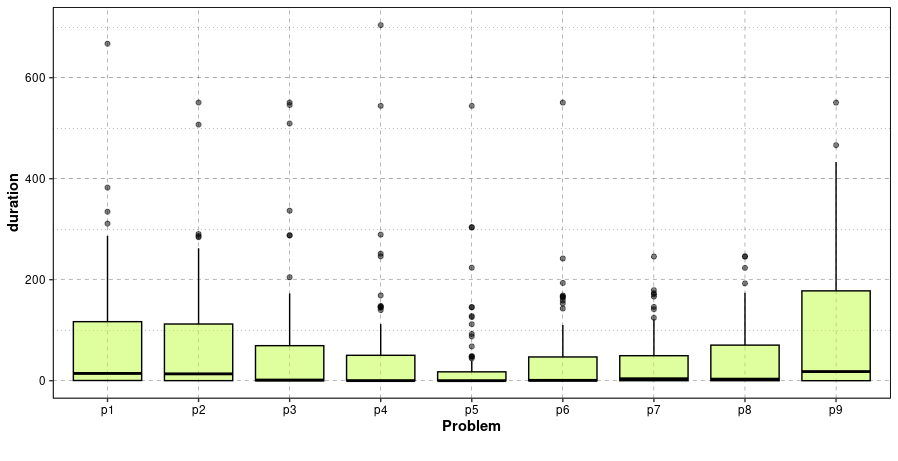
\includegraphics[width=0.8\textwidth]{análisis/boxplotduration.png}
    \caption{Boxplots del tiempo necesario para resolver cada uno de los problemas.}
    \label{fig:boxplotduration}
\end{figure}

Podemos ver un resumen del test ANOVA de un factor en el Cuadro \ref{tab:ANOVAduration}. De nuevo, los tests detectan comportamientos diferentes: obtenemos $p=0.0074$ con el test ANOVA de un solo factor y $p=0.0002763$ con la prueba de Kruskal-Wallis).

% latex table generated in R 4.3.1 by xtable 1.8-4 package
% Wed Aug  2 18:33:43 2023
\begin{table}[H]
\centering
\caption{Resultados del test ANOVA de un solo factor (tiempo en resolver los problemas por primera vez).}
\label{tab:ANOVAduration}
\begin{tabular}{lrrrrr}
  \hline
 & Df & Sum Sq & Mean Sq & F value & Pr($>$F) \\ 
  \hline
duration & 8 & 222548.19 & 27818.52 & 2.64 & 0.0074 \\ 
  Residuals           & 642 & 6757495.31 & 10525.69 &  &  \\ 
   \hline
\end{tabular}
\end{table}

Adicionalmente, se aportan los resultados del test de Tukey por pares de problemas (Cuadro \ref{tab:Tukeyduration}). En ellos se detecta, por ejemplo, que los pares de problemas $P9-P7$ y $P9-P5$ son estadísticamente diferentes ($\text{p adj} = 0.02$ en ambos casos). En la Figura \ref{fig:confidenceduration} se muestran los intervalos de confianza de todas las diferencias entre las distintas parejas de años.

% latex table generated in R 4.3.1 by xtable 1.8-4 package
% Wed Aug  2 18:34:46 2023
\begin{table}[H]
\centering
\caption{Test HSD de Tukey (Honestly-significance-difference) del tiempo de resolución por problemas.}
\label{tab:Tukeyduration}
\begin{tabular}{rrrrr}
  \hline
 & diff & lwr & upr & p adj \\ 
  \hline
p2-p1 & -8.38 & -59.84 & 43.08 & 1.00 \\ 
  p3-p1 & -14.68 & -66.66 & 37.31 & 0.99 \\ 
  p4-p1 & -22.83 & -74.99 & 29.33 & 0.91 \\ 
  p5-p1 & -41.17 & -92.97 & 10.63 & 0.25 \\ 
  p6-p1 & -34.32 & -86.85 & 18.22 & 0.52 \\ 
  p7-p1 & -41.10 & -93.26 & 11.07 & 0.26 \\ 
  p8-p1 & -27.84 & -80.38 & 24.70 & 0.78 \\ 
  p9-p1 & 19.54 & -35.45 & 74.52 & 0.97 \\ 
  p3-p2 & -6.30 & -58.28 & 45.68 & 1.00 \\ 
  p4-p2 & -14.45 & -66.61 & 37.71 & 0.99 \\ 
  p5-p2 & -32.79 & -84.60 & 19.01 & 0.56 \\ 
  p6-p2 & -25.94 & -78.48 & 26.60 & 0.84 \\ 
  p7-p2 & -32.72 & -84.88 & 19.45 & 0.58 \\ 
  p8-p2 & -19.46 & -72.00 & 33.07 & 0.97 \\ 
  p9-p2 & 27.91 & -27.07 & 82.90 & 0.82 \\ 
  p4-p3 & -8.15 & -60.83 & 44.52 & 1.00 \\ 
  p5-p3 & -26.49 & -78.81 & 25.83 & 0.82 \\ 
  p6-p3 & -19.64 & -72.69 & 33.41 & 0.97 \\ 
  p7-p3 & -26.42 & -79.10 & 26.25 & 0.83 \\ 
  p8-p3 & -13.17 & -66.21 & 39.88 & 1.00 \\ 
  p9-p3 & 34.21 & -21.26 & 89.68 & 0.60 \\ 
  p5-p4 & -18.34 & -70.84 & 34.16 & 0.98 \\ 
  p6-p4 & -11.49 & -64.71 & 41.74 & 1.00 \\ 
  p7-p4 & -18.27 & -71.12 & 34.59 & 0.98 \\ 
  p8-p4 & -5.01 & -58.24 & 48.21 & 1.00 \\ 
  p9-p4 & 42.36 & -13.28 & 98.01 & 0.30 \\ 
  p6-p5 & 6.85 & -46.02 & 59.73 & 1.00 \\ 
  p7-p5 & 0.07 & -52.43 & 52.57 & 1.00 \\ 
  p8-p5 & 13.33 & -39.55 & 66.20 & 1.00 \\ 
  p9-p5 & 60.70 & 5.40 & 116.01 & 0.02 \\ 
  p7-p6 & -6.78 & -60.00 & 46.45 & 1.00 \\ 
  p8-p6 & 6.47 & -47.12 & 60.07 & 1.00 \\ 
  p9-p6 & 53.85 & -2.14 & 109.85 & 0.07 \\ 
  p8-p7 & 13.25 & -39.97 & 66.48 & 1.00 \\ 
  p9-p7 & 60.63 & 4.99 & 116.27 & 0.02 \\ 
  p9-p8 & 47.38 & -8.62 & 103.37 & 0.17 \\ 
   \hline
\end{tabular}
\end{table}

\begin{figure}[H]
    \centering
    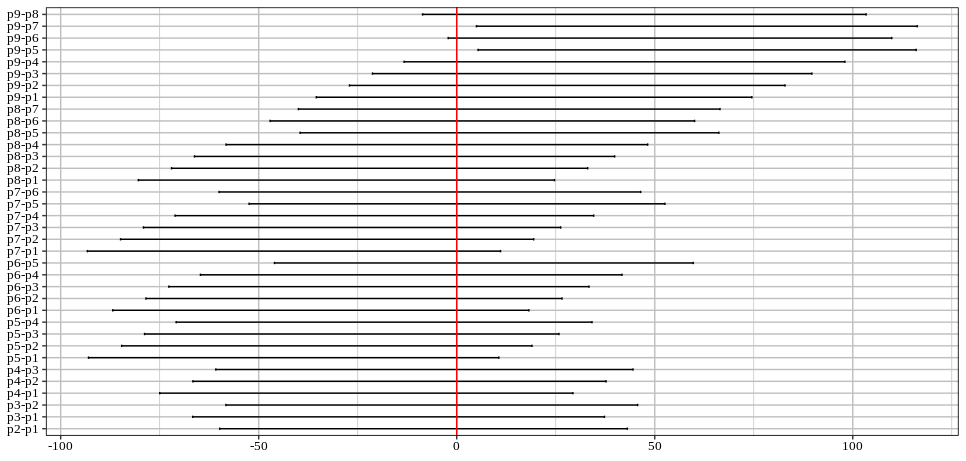
\includegraphics[width=0.80\textwidth]{análisis/confidenceduration.png}
    \caption{Intervalos de confianza del tiempo empleado en la resolución de los problemas propuestos por primera vez.}
    \label{fig:confidenceduration}
\end{figure}

Por lo tanto, se puede ver, dadas las evidencias aportadas, que la resolución de cada problema exige respuestas claramente diferentes por parte del alumnado.

\section{Actividad registrada}\label{sec:activityrecorded}

El número de registros y de sesiones de trabajo de cada uno de los años analizados se muestran en el Cuadro \ref{tab:records}. Como podemos ver, aunque el curso académico 2020-2021 (Y2020) registra más actividad que los demás, no es el que presenta el mayor número de sesiones.

\begin{table}[H]
\centering
\caption{Número de registros y sesiones almacenados en el servidor por años.}
\label{tab:records}
\begin{tabular}{ccc}
\hline
\textbf{Year}  & \textbf{Activity Records} & \textbf{Sessions}  \\ \hline
Y2015 & 12088            &  4489  \\
Y2016 & 12525            &  4538  \\
Y2017 & 9088             &  3661  \\
Y2018 & 5705             &  2811  \\
Y2019 & 14475            &  5156  \\
Y2020 & 21188            &  3904  \\
Y2021 & 11961            &  6113  \\ \hline
Mean & 12432.86 & 4381.714 \\
SD & 4789.312 & 1068.3 \\ \hline
\end{tabular}
\end{table}

Al ser un servicio $24$ horas los $7$ días de la semana, los alumnos interactúan con el laboratorio remoto en cualquier día de la semana tal y como puede verse en la Figura \ref{fig:days} y a cualquier hora del día (Figura \ref{fig:hours}). Así pues, el uso intensivo del servidor por parte del alumnado aporta solidez y fiabilidad al dataset que estamos considerando.

\begin{figure}[H]
\centering
\subfloat[Histograma de los días de la semana.]{\label{fig:days}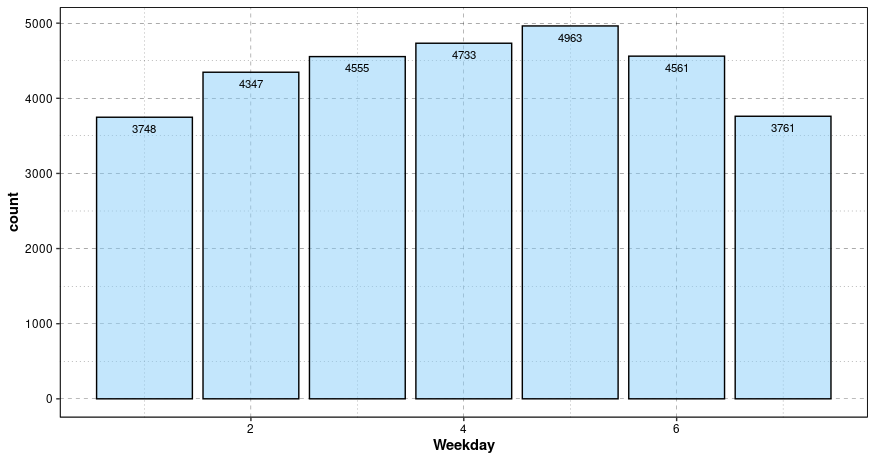
\includegraphics[width=0.9\textwidth]{análisis/days.png}}\\
\subfloat[Histograma de las horas del día.]{\label{fig:hours}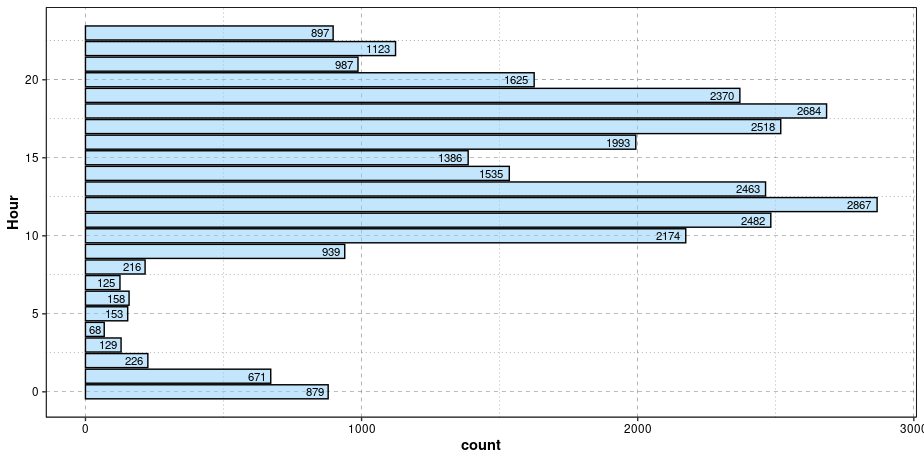
\includegraphics[width=0.9\textwidth]{análisis/hours.png}}
\caption{Actividad registrada en el servidor remoto.}
\label{fig:activity}
\end{figure}

El número y tipo de las sesiones de trabajo de cada uno de los grupos puede contemplarse en el Cuadro \ref{tab:type}.

\subsection{Análisis de la normalidad de la distribución del número de sesiones}\label{sec:NormalityNumSessions}

En las Figuras \ref{fig:boxplotresiduals} y \ref{fig:histogramresiduals} podemos ver el boxplot de los residuos de la variable número de sesiones (\emph{s}) junto con el histograma de los mismos.

\begin{figure}[H]
\centering
\subfloat[Boxplot de los residuos del número de sesiones.]{\label{fig:boxplotresiduals}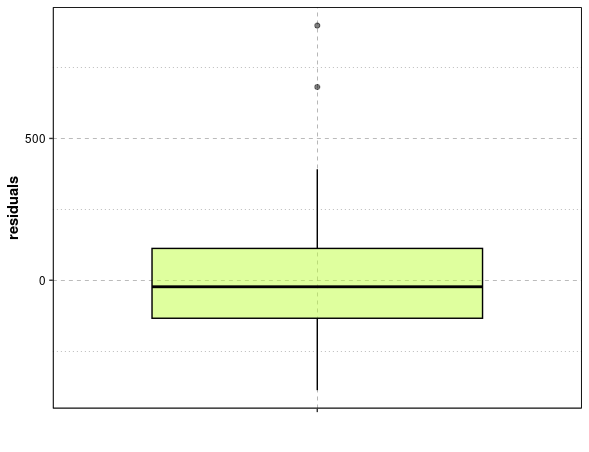
\includegraphics[width=0.47\textwidth]{análisis/residualss.png}}\qquad
\subfloat[Histograma de los residuos del número de sesiones.]{\label{fig:histogramresiduals}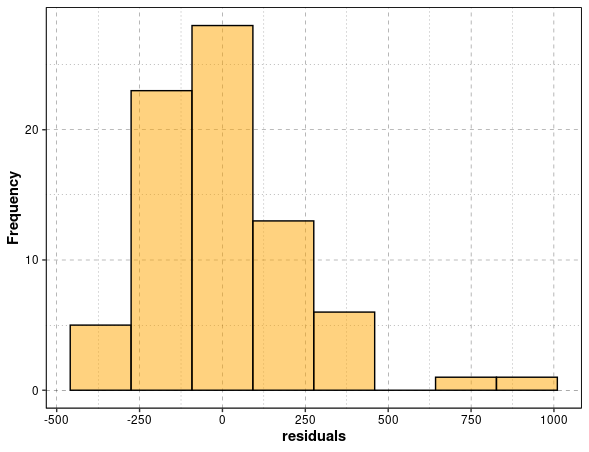
\includegraphics[width=0.47\textwidth]{análisis/histograms.png}}
\caption{Distribución de los residuos del número de sesiones.}
\label{fig:activity}
\end{figure}

A continuación, en las Figuras \ref{fig:densitysessions} y \ref{fig:q-qsessions}, podemos observar que la distribución del número de sesiones no es perfectamente normal pero es casi-normal si eliminamos algunos outliers. La línea discontinua vertical marca el valor más probable ($336$ sesiones), lo que muestra un gran esfuerzo por parte del alumnado teniendo en cuenta la duración de la práctica (Cuadro \ref{tab:days}).

\begin{figure}[H]
    \centering
    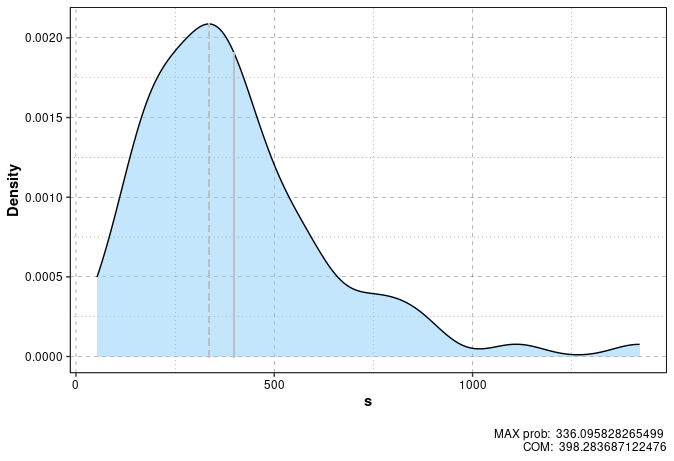
\includegraphics[width=0.70\textwidth]{análisis/densitys.png}
    \caption{Función de densidad de probabilidad del número de sesiones.}
    \label{fig:densitysessions}
\end{figure}


\begin{figure}[H]
    \centering
    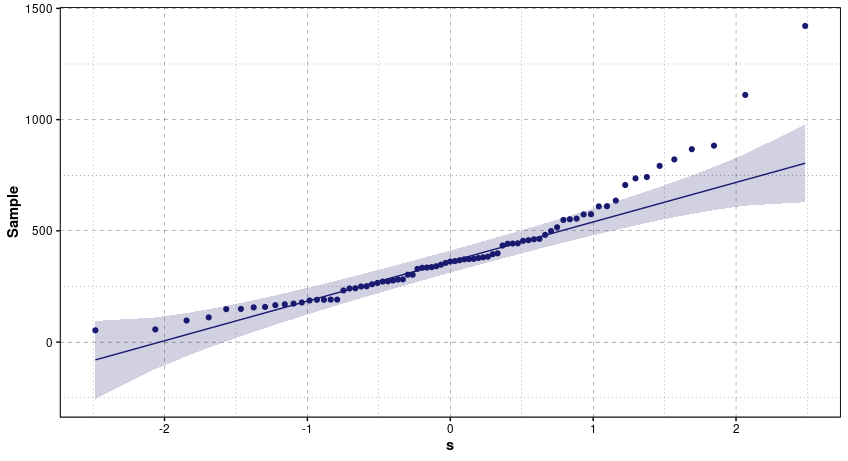
\includegraphics[width=0.75\textwidth]{análisis/qqplots.png}
    \caption{Gráfico Q-Q del número de sesiones.}
    \label{fig:q-qsessions}
\end{figure}

Además, podemos ver en la Figura \ref{fig:outlierss} que hay algunos outliers ($867$, $883$, $1421$ y $1111$) considerando la distribución del número total de sesiones por grupo de alumnos. Segmentando por años, obtenemos los boxplots que se muestran en la Figura \ref{fig:boxplotsessionsyearinitial}. Así pues, eliminaremos aquellos registros que sean outliers en todos los años. Tras realizar la acción anterior, obtenemos la distribución del número de sesiones que se muestra en la Figura \ref{fig:outlierss2}.

\begin{figure}[H]
    \centering
    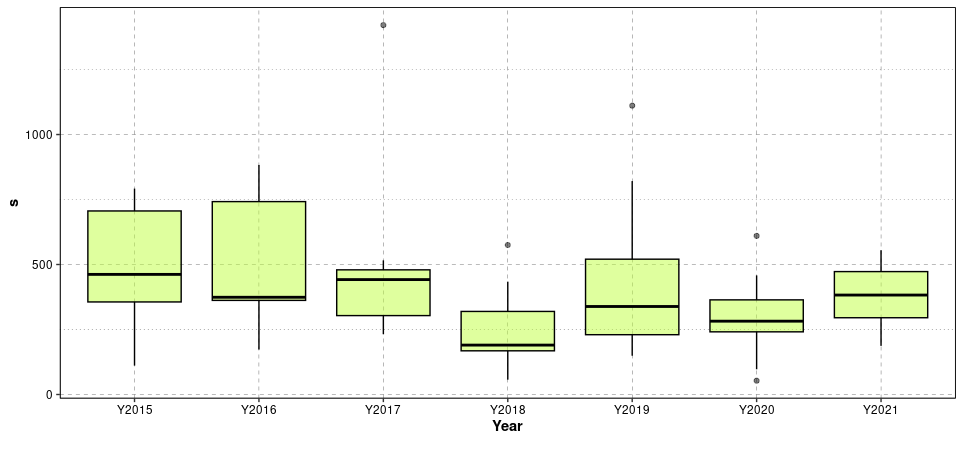
\includegraphics[width=0.80\textwidth]{análisis/boxplotinitials.png}
    \caption{Boxplot del número de sesiones por año inicialmente.}
    \label{fig:boxplotsessionsyearinitial}
\end{figure}

\begin{figure}[H]
    \centering
    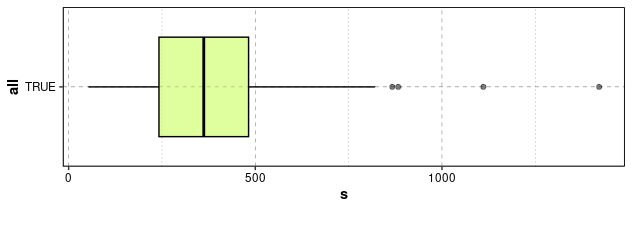
\includegraphics[width=0.60\textwidth]{análisis/outlierss.png}
    \caption{Distribución del número de sesiones inicial.}
    \label{fig:outlierss}
\end{figure}

\begin{figure}[H]
    \centering
    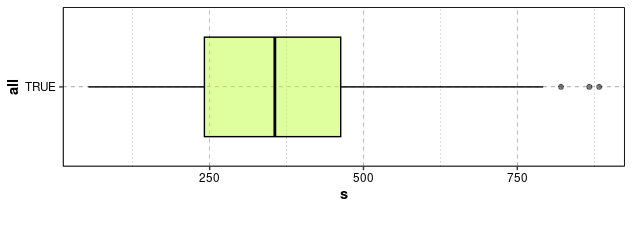
\includegraphics[width=0.60\textwidth]{análisis/outlierss2.png}
    \caption{Distribución del número de sesiones tras la eliminación de algunos outliers.}
    \label{fig:outlierss2}
\end{figure}

Examinamos ahora los bloques significativos entre ellos agrupando los datos en ocho particiones mediante el algoritmo de las K-medias, tal y como se muestra en la Figura \ref{fig:KMeans8}. Los resultados obtenidos pueden verse en las Figuras \ref{fig:KMeans8boxplot} y \ref{fig:KMeans8count}.

\begin{figure}[H]
    \centering
    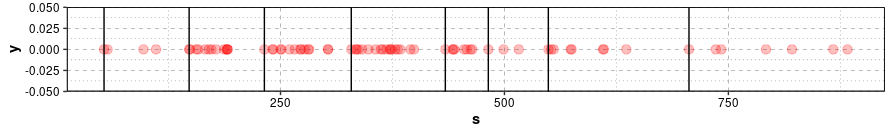
\includegraphics[width=0.6\textwidth]{análisis/KMeanss8.png}
    \caption{Particiones obtenidas con $K = 8$.}
    \label{fig:KMeans8}
\end{figure}

\begin{figure}[H]
\centering
\subfloat[Boxplot de cada una de las particiones.]{\label{fig:KMeans8boxplot}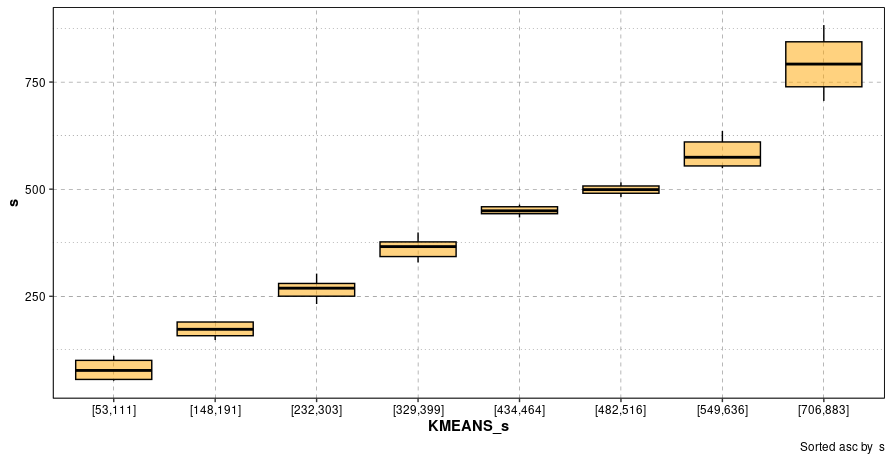
\includegraphics[width=0.47\textwidth]{análisis/KMeanssboxplot.png}}\qquad
\subfloat[Número de grupos por partición.]{\label{fig:KMeans8count}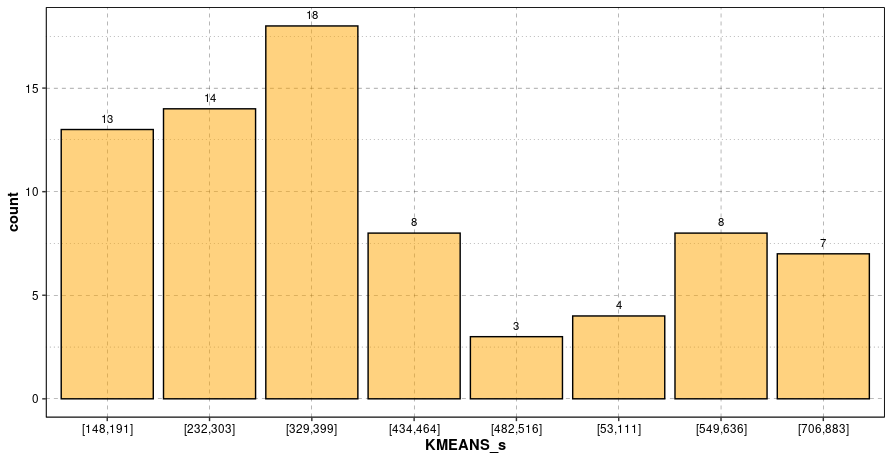
\includegraphics[width=0.47\textwidth]{análisis/KMeansscount.png}}%
\caption{Resultados obtenidos tras aplicar el algoritmo de las $K$-Medias con $K = 8$.}
\label{fig:KMeans8details}
\end{figure}

Nótese que como hemos una obtenido una precisión del $97.95579\% > 95\%$, no eliminaremos más outliers.

Así pues, tras la eliminación de los outliers correspondientes tanto al número de sesiones como al número de problemas resueltos como veremos en la subsección \ref{sec:NumProblems} (podemos ver la nueva función de densidad en la Figura \ref{fig:normalitys}) se procede a aplicar el test de normalidad de Shapiro-Wilk. Como se obtiene $p-value = 0.003307 < 0.05$, podemos decir que estadísticamente no sigue una distribución normal. No obstante, teniendo en cuenta que el tamaño de la muestra es relativamente pequeño (tenemos un total de $77$ grupos de prácticas), podemos considerar que se trata de una distribución normal.

\begin{figure}[H]
    \centering
    \includegraphics[width=0.70\textwidth]{análisis/normalitys.png}
    \caption{Función de densidad de probabilidad del número de sesiones tras eliminar algunos outliers.}
    \label{fig:normalitys}
\end{figure}

\subsection{Sesiones por cada problema}

En la Figura \ref{fig:boxplotsessionsproblem} podemos ver el boxplot del número de sesiones por problema. Como podemos ver, el problema P1 es mucho más frecuentado que el resto. No obstante, la diferencia entre el número de sesiones abiertas del problema P1 y el número de sesiones abiertas de los problemas restantes se debe a que los alumnos utilizan el primer problema como base de todos los experimentos y para testear las comunicaciones con el servidor. Así pues, el problema P1 es frecuentemente utilizado, no ya sólo al comienzo de la práctica, sino durante todo el desarrollo de la misma.

\begin{figure}[H]
    \centering
    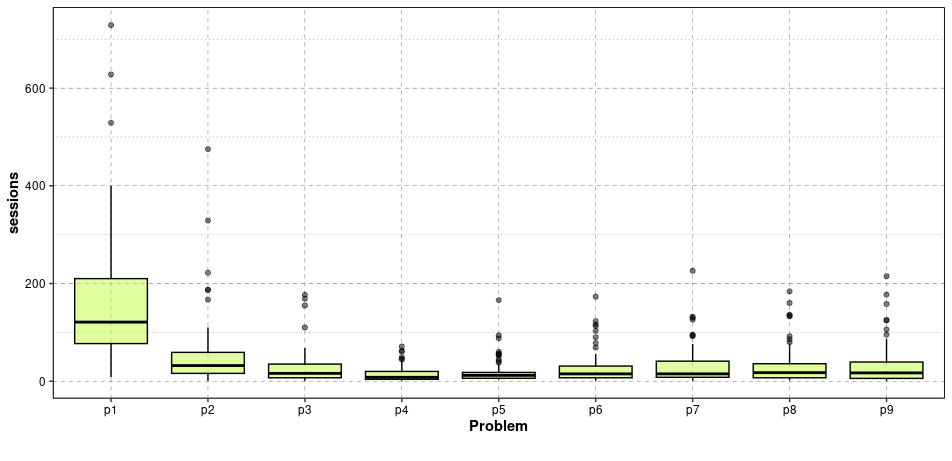
\includegraphics[width=0.8\textwidth]{análisis/boxplotsessionsproblem.png}
    \caption{Boxplot del número de sesiones por problema.}
    \label{fig:boxplotsessionsproblem}
\end{figure}

\subsection{Sesiones cada año}\label{sec:ANOVANumSessions}

En la Figura \ref{fig:boxplotsessionsyear} podemos ver los boxplots de las sesiones de trabajo abiertas en el servidor año tras año. A continuación, se procederá a demostrar que el número de sesiones sigue la misma distribución de probabilidad todos los años. Es decir, veremos que la variabilidad perceptible en la Figura \ref{fig:boxplotsessionsyear} se debe al azar.

\begin{figure}[H]
    \centering
    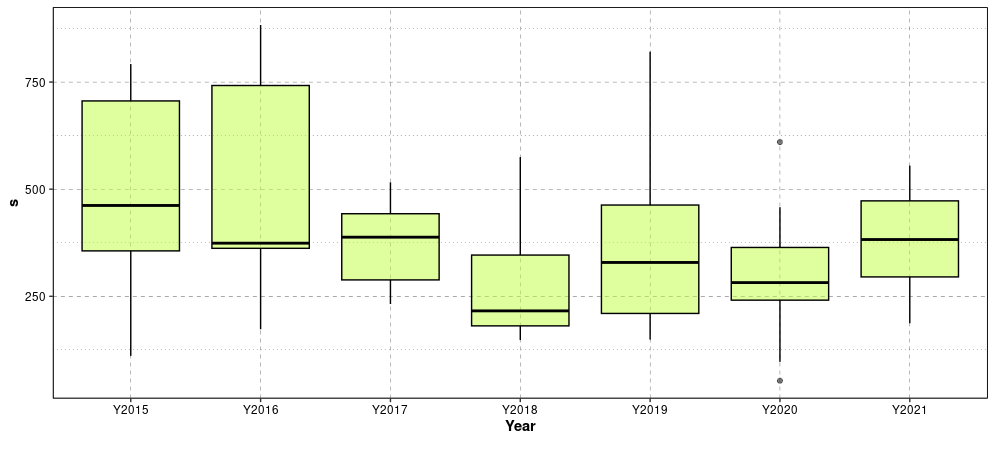
\includegraphics[width=0.80\textwidth]{análisis/boxplotfinals.png}
    \caption{Boxplot del número de sesiones por año tras la eliminación de algunos outliers.}
    \label{fig:boxplotsessionsyear}
\end{figure}

Un resumen de los resultados obtenidos al realizar el test ANOVA se muestra en el Cuadro \ref{tab:ANOVAnumsessions}. La hipótesis nula establece que el número de sesiones medio de los siete cursos académicos estudiados es el mismo. Así pues, estableciendo un nivel de significancia de $0.05$, como tenemos que $p = 0.0412 < 0.05$, por lo que las diferencias entre las medias podrían ser estadísticamente significativas. Aplicando el test de Kruskal-Wallis, obtenemos un $p-value$ igual a $0.08798 > 0.05$.

% latex table generated in R 4.3.0 by xtable 1.8-4 package
% Sat May 27 18:26:28 2023
\begin{table}[H]
\centering
\caption{Resultados del test ANOVA de un solo factor (número de sesiones).}
\label{tab:ANOVAnumsessions}
\begin{tabular}{lrrrrr}
  \hline
 & Df & Sum Sq & Mean Sq & F value & Pr($>$F) \\ 
  \hline
s & 6 & 460434.32 & 76739.05 & 2.34 & 0.0412 \\ 
  Residuals         & 67 & 2197451.96 & 32797.79 &  &  \\ 
   \hline
\end{tabular}
\end{table}

Además, se ha realizado un test de Tukey por pares de años (Cuadro \ref{tab:Tukeynumsessions}). En él se observa que todos los pares pueden considerarse estadísticamente iguales ($\text{p adj} > 0.1$ en todos ellos). Así pues, podemos concluir que el número de sesiones abiertas en el servidor sigue la misma distribución de probabilidad año tras año.

La Figura \ref{fig:confidencenumsessions} muestra los intervalos de confianza de todas las diferencias entre las distintas parejas de años. Así pues, consideraremos que el número de sesiones de cada grupo por año es equivalente (las variaciones son debidas al azar). Esto es importante porque indica que el comportamiento más básico de los alumnos, que viene dado por cuántas veces se conectan al servidor, es el mismo en todos los cursos académicos considerados.

% latex table generated in R 4.3.0 by xtable 1.8-4 package
% Sat May 27 18:26:44 2023
\begin{table}[H]
\centering
\caption{Test HSD de Tukey (Honestly-significance-difference) del número de sesiones por años.}
\label{tab:Tukeynumsessions}
\begin{tabular}{rrrrr}
  \hline
 & diff & lwr & upr & p adj \\ 
  \hline
Y2016-Y2015 & 5.44 & -254.06 & 264.95 & 1.00 \\ 
  Y2017-Y2015 & -125.44 & -415.58 & 164.69 & 0.84 \\ 
  Y2018-Y2015 & -223.38 & -476.31 & 29.56 & 0.12 \\ 
  Y2019-Y2015 & -131.05 & -378.48 & 116.38 & 0.68 \\ 
  Y2020-Y2015 & -198.78 & -437.49 & 39.93 & 0.16 \\ 
  Y2021-Y2015 & -116.72 & -346.09 & 112.66 & 0.72 \\ 
  Y2017-Y2016 & -130.89 & -421.03 & 159.25 & 0.81 \\ 
  Y2018-Y2016 & -228.82 & -481.76 & 24.11 & 0.10 \\ 
  Y2019-Y2016 & -136.49 & -383.92 & 110.93 & 0.63 \\ 
  Y2020-Y2016 & -204.22 & -442.93 & 34.49 & 0.14 \\ 
  Y2021-Y2016 & -122.16 & -351.53 & 107.21 & 0.67 \\ 
  Y2018-Y2017 & -97.93 & -382.21 & 186.34 & 0.94 \\ 
  Y2019-Y2017 & -5.61 & -284.99 & 273.78 & 1.00 \\ 
  Y2020-Y2017 & -73.33 & -345.03 & 198.36 & 0.98 \\ 
  Y2021-Y2017 & 8.73 & -254.80 & 272.26 & 1.00 \\ 
  Y2019-Y2018 & 92.33 & -148.20 & 332.86 & 0.90 \\ 
  Y2020-Y2018 & 24.60 & -206.95 & 256.15 & 1.00 \\ 
  Y2021-Y2018 & 106.66 & -115.25 & 328.57 & 0.77 \\ 
  Y2020-Y2019 & -67.73 & -293.25 & 157.80 & 0.97 \\ 
  Y2021-Y2019 & 14.34 & -201.28 & 229.95 & 1.00 \\ 
  Y2021-Y2020 & 82.06 & -123.49 & 287.61 & 0.89 \\ 
   \hline
\end{tabular}
\end{table}

\begin{figure}[H]
    \centering
    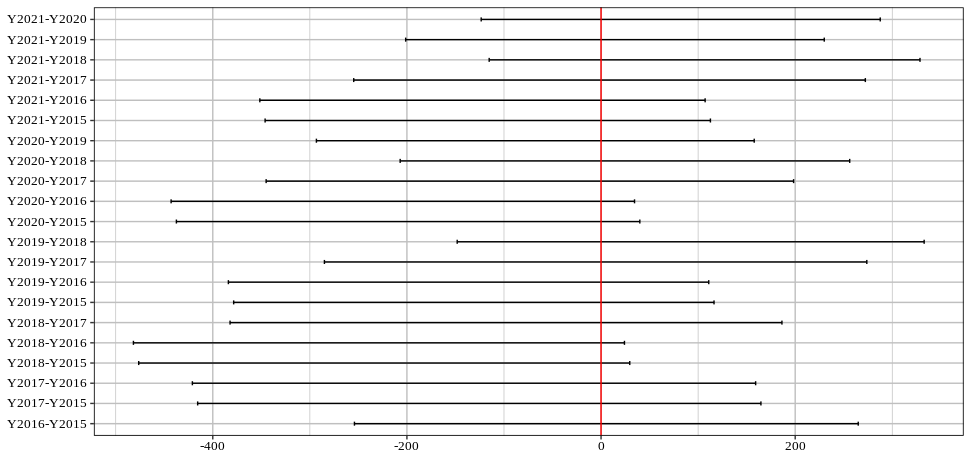
\includegraphics[width=0.80\textwidth]{análisis/confidences.png}
    \caption{Intervalos de confianza del número de sesiones por años.}
    \label{fig:confidencenumsessions}
\end{figure}

\subsection{Análisis de la distribución del número de problemas resueltos}\label{sec:NumProblems}

Además, a partir de los registros almacenados en el servidor se calcularán el número de problemas resueltos por cada grupo de prácticas. Como se puede intuir, se tratará de una variable discreta. En la Figura \ref{fig:initialp} podemos ver que el número de problemas resueltos oscila entre $6$ y $9$.

\begin{figure}[H]
    \centering
    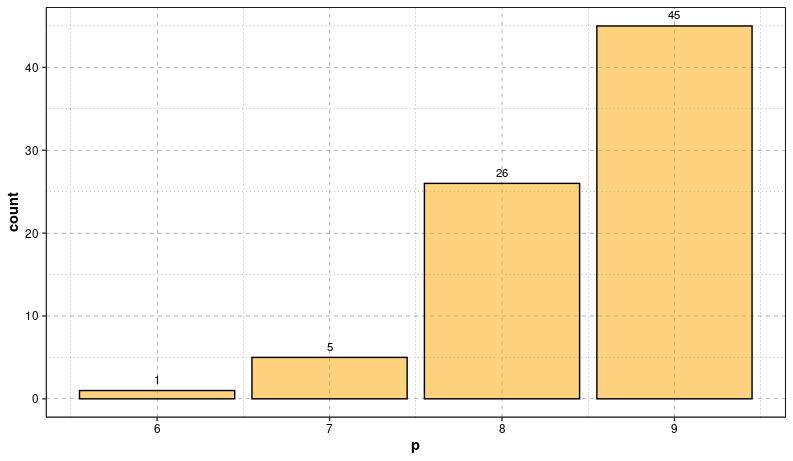
\includegraphics[width=0.6\textwidth]{rendimiento/initialp.png}
    \caption{Distribución del número de problemas resueltos.}
    \label{fig:initialp}
\end{figure}

Adicionalmente, podemos observar en la Figura \ref{fig:outliersp} la existencia de un elemento extremo ($6$) en la distribución del número de problemas resueltos por grupo de alumnos. Segmentando por años, obtenemos los boxplots que se muestran en la Figura \ref{fig:boxplotproblemsyear}. Así pues, eliminaremos el outlier encontrado puesto que se trata de un valor extremo en todos los años incluidos en este estudio.

\begin{figure}[H]
    \centering
    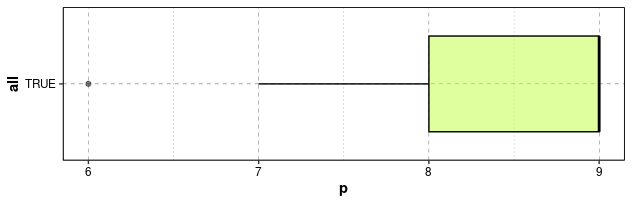
\includegraphics[width=0.60\textwidth]{análisis/outliersp.png}
    \caption{Distribución del número de problemas resueltos inicial.}
    \label{fig:outliersp}
\end{figure}

\begin{figure}[H]
    \centering
    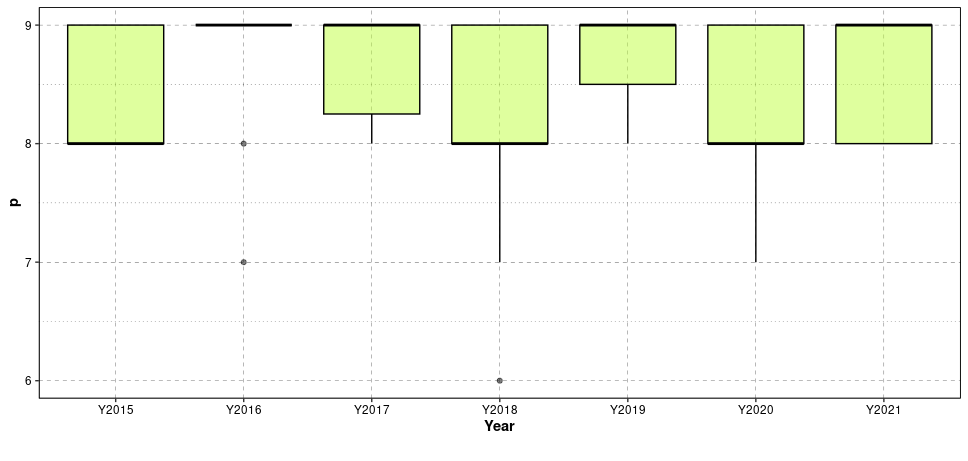
\includegraphics[width=0.80\textwidth]{análisis/boxplotinitialp.png}
    \caption{Boxplot del número de problemas resueltos por año.}
    \label{fig:boxplotproblemsyear}
\end{figure}

A pesar de que el estudio descriptivo anterior muestra unos datos muy variados, casi todos ellos son homogéneos año tras año. Es decir, todos los años son diferentes pero las variables recogidas año tras año presentan la misma distribución de probabilidad. No obstante, el objetivo de este estudio es sentar las bases para conseguir una experiencia de aprendizaje óptima para todos los grupos de alumnos. Así pues, se va a poner énfasis en detectar a aquellos grupos que estén en riesgo de obtener un peor rendimiento o peores calificaciones.